
\chapter{Experimento 2}
    

    \section{Methodology (generated)}

        \subsection{Overview}

            This chapter describes the experimental methodology used to evaluate large language model (LLM) agents and workflows for answering questions in the oil well operations domain. The experiment integrates multiple LLM configurations, agent architectures, and retrieval-augmented generation (RAG) tools, leveraging Petrobras datasets.

            [POR ÚLTIMO, INSERIR OBJETIVOS DO EXPERIMENTO E HIPOTESES]
            \textit{<insert brief summary of research objectives and hypotheses here>}

        \subsection{Experimental Workflow}

            \subsubsection{Dataset Preparation}

                The experimental workflow was designed to provide a thorough and reproducible evaluation of language model agents within oil well operations. The process begins with the careful preparation of the dataset, which is composed of questions and corresponding ground truth answers derived from a diverse range of operational records, incident reports, and lessons learned. To ensure the quality and relevance of the data, questions undergo a filtering and preprocessing phase where clarity, diversity, and alignment with real-world scenarios are prioritized. This includes removing duplicates, standardizing terminology, and confirming that each question is properly paired with an accurate answer. The dataset is further validated for completeness and consistency, ensuring it represents the full spectrum of operational challenges, such as safety, cementing, and intervention scenarios.

            \subsubsection{Model and Setup Selection}

                Following dataset preparation, the experimental design incorporates a variety of agent architectures. These include approaches where questions are routed to specialized agents, single-agent systems that centralize all reasoning and retrieval, and multi-agent frameworks that leverage collaboration among specialized agents under a supervisory structure. Each of these configurations is evaluated using different language models, allowing for a comprehensive assessment of how model choice and agent setup influence performance. The agents are also provided with access to advanced retrieval tools and domain-specific knowledge bases, enabling them to draw on a broad foundation of operational expertise.

            \subsubsection{Execution Loop}

                The core of the experimental workflow is an execution loop depicted in Algorithm~\ref{alg:execution_loop}. For each combination of question, agent setup, and language model, the system systematically loads the relevant data, configures the agent, and executes the workflow. Throughout this process, all responses and intermediate reasoning steps are meticulously logged. This approach not only ensures systematic coverage of all experimental conditions but also provides full traceability for subsequent analysis. The automation of these procedures guarantees consistency and reproducibility, while the comprehensive logging facilitates in-depth evaluation and comparison of agent performance across a range of operational scenarios.

            
                \begin{algorithm}
                    \caption{Experiment Execution Loop}
                    \begin{algorithmic}[1]
                    \Require questions, setups, models
                    \Ensure results
                    
                    \Function{RunExperiment}{}
                        \State $results \gets \{\}$
                        
                        \ForAll{$question \in questions$}
                            \State $ground\_truth \gets question.ground\_truth$
                            
                            \ForAll{$setup \in setups$}
                                \ForAll{$model \in models$}
                                    \State $agent \gets \text{InitializeAgent}(setup, model)$
                                    \State $response \gets agent.\text{ProcessQuestion}(question)$
                                    
                                    \State $metrics \gets \text{EvaluateResponse}(response, ground\_truth)$
                                    
                                    \State $results[question, setup, model] \gets \{$
                                    \State \hspace{1cm} $"response": response,$
                                    \State \hspace{1cm} $"metrics": metrics,$
                                    \State \hspace{1cm} $"execution\_trace": agent.trace$
                                    \State $\}$
                                \EndFor
                            \EndFor
                        \EndFor
                        
                        \State \Return $\text{AggregateResults}(results)$
                    \EndFunction
                    
                    \end{algorithmic}
                    \label{alg:execution_loop}
                \end{algorithm}
            
            \subsubsection{Evaluation and Metrics}

                Following the execution of all experimental combinations, a comprehensive evaluation framework is applied to assess agent performance. The system calculates a suite of quantitative metrics for each question, setup, and model combination by comparing the generated answers against the established ground truth. These metrics include standard performance indicators such as accuracy, precision, recall, and F1 score, which provide a multifaceted view of response quality. For open-ended questions where binary correctness measures are insufficient, a confusion matrix approach is implemented to capture nuances in answer quality and content coverage. Additionally, the system measures answer size ratio relative to ground truth, offering insights into model verbosity and conciseness. These metrics are then aggregated across different dimensions to enable meaningful comparisons between agent architectures and language models, revealing patterns in performance across various operational scenarios and question types.

            \subsubsection{Reproducibility and Quality Control}

                To ensure scientific rigor and reproducibility, the experimental methodology incorporates robust tracking of all environmental variables and configuration parameters. The system maintains detailed logs of the computational environment, including software versions, dependency specifications, and hardware characteristics that might influence results. All experimental parameters, from model identifiers to dataset specifications, are systematically recorded alongside the results they generate. Throughout the experimental process, periodic validation checks are performed to maintain data integrity and result consistency, with anomalies flagged for investigation. This comprehensive approach to reproducibility not only facilitates verification of findings but also enables future extensions of the research with comparable baselines. The quality control measures embedded in the workflow ensure that conclusions drawn from the experiments rest on a foundation of methodological soundness and data reliability.

            \textit{<insert workflow diagram or pseudocode here to illustrate the above stages>}

        \subsection{Data Sources}

                The experimental evaluation relies on a carefully curated collection of data sources that represent the diverse knowledge domains relevant to oil well operations. At the core of the experiment is a comprehensive questions dataset containing structured entries that simulate real-world queries an operator might encounter. This dataset was developed through extensive collaboration with domain experts and analysis of historical operational records. Each entry in the dataset contains a question formulated in natural language, a unique identifier, categorical metadata to facilitate analysis, and a corresponding ground truth answer validated by subject matter experts. The questions span various complexity levels, from factual inquiries to complex reasoning scenarios that require integration of multiple knowledge sources.

            To provide the language models with the necessary domain knowledge, the experiment incorporates several specialized knowledge bases that reflect different aspects of oil well operations:

            \begin{itemize}
                \item \textbf{Knowledge Bases and Tools}:
                \begin{itemize}
                    \item \textbf{Lessons}: A repository of knowledge items capturing insights, best practices, and technical know-how from past oil well operations. These lessons represent institutional memory and expertise accumulated over years of operational experience.
                    \item \textbf{Alertas SMS}: A collection of safety alerts and incident reports documenting past events, near-misses, and accidents, providing critical safety information and preventative measures.
                    \item \textbf{Cronoweb}: A comprehensive database of scheduling information and intervention records, detailing maintenance activities, equipment deployments, and operational timelines.
                    \item \textbf{SITOP}: Detailed daily operational logs from drilling rigs, containing technical parameters, operational decisions, and situational reports from active drilling operations.
                \end{itemize}
            \end{itemize}

            These knowledge sources were preprocessed to ensure consistency, remove sensitive information, and optimize retrieval performance. The integration of these diverse data sources enables a holistic evaluation of how language model agents navigate the complex informational landscape of oil well operations, from technical specifications to safety protocols and historical precedents.

            \textit{<insert table or image summarizing datasets and tools here>}

        \subsection{System Architecture}

                The experimental system was implemented using modern Python frameworks specialized for language model orchestration and agent workflows. The architecture leverages the LangChain and LangGraph ecosystems, which provide robust foundations for building complex language model applications with multiple components and state management. This subsection details the modular design of the system, highlighting how different components interact to enable systematic evaluation of language model agents in oil well operations.

            \subsubsection{Experiment Orchestration}

                At the core of the system architecture is an experiment orchestration layer responsible for coordinating the entire evaluation process. This component manages the loading of questions from the dataset, systematically iterates through different model and setup combinations, and ensures proper logging of results. The orchestrator maintains experiment state across multiple runs, handles error recovery, and implements checkpointing to allow for resumption of long-running experiments. By centralizing control flow, this component ensures that all experimental conditions are tested consistently and that results are captured in a standardized format for subsequent analysis.

            \subsubsection{Agent Workflow Frameworks}

                The system implements multiple agent workflow frameworks to evaluate different approaches to question answering in the oil well domain. These frameworks define the flow of information and decision-making processes within and between language model agents. The implemented workflows include a Linear-Flow with Router (CORTEX) that directs questions to specialized processing paths, a Single-Agent approach that centralizes all reasoning and tool use, and a Multi-Agent Supervisor framework that coordinates multiple specialized agents. Each workflow is defined declaratively, specifying the sequence of operations, decision points, and information exchange patterns that govern agent behavior during question processing.

            \subsubsection{Nodes and Tool Integration}

                The system architecture includes specialized nodes that implement specific reasoning steps and tool-calling logic. These nodes serve as the building blocks of agent workflows, encapsulating discrete functionality such as question analysis, knowledge retrieval, and answer synthesis. The tool integration layer provides agents with access to external knowledge sources through a standardized interface, enabling semantic search over domain-specific corpora, structured data queries, and other specialized operations. This modular approach to tool integration allows for consistent evaluation of how different agent architectures leverage available tools and knowledge sources.

            \subsubsection{Prompt Engineering and System Messages}

                A critical component of the architecture is the prompt engineering layer, which defines the instructions and context provided to language models. This includes carefully crafted system messages that establish the role and capabilities of each agent, prompt templates that structure inputs consistently across experimental conditions, and few-shot examples that guide model behavior. The system maintains a library of prompt variants optimized for different tasks within the question-answering workflow, ensuring that each agent receives appropriate guidance while maintaining experimental control.

            \subsubsection{State Management and Metrics}

                The architecture incorporates a comprehensive state management system that tracks the progress of experiments, maintains contextual information across agent interactions, and captures intermediate reasoning steps. This component is tightly integrated with the metrics calculation subsystem, which computes performance indicators in real-time as experiments progress. The metrics framework implements various evaluation approaches, from simple accuracy measures to sophisticated semantic similarity calculations, providing multi-dimensional assessment of agent performance. All experimental data, including intermediate states and final results, is persisted in structured formats to enable both immediate feedback and in-depth post-experiment analysis.

                \textit{<insert system architecture diagram here>}

        \subsection{Experimental Setups}

            To comprehensively evaluate language model performance in well construction operations, the experiment employed multiple agent architectures and model configurations. This subsection details the different experimental setups, highlighting their design principles, operational characteristics, and the rationale behind their selection. The experimental design deliberately incorporates contrasting approaches to agent architecture, enabling comparative analysis of different strategies for complex question answering in specialized domains.
            

            \subsubsection{Linear-Flow}

                The Linear-Flow architecture represents the simplest RAG design, where user input is processed in a strictly sequential manner. 

                \begin{figure}[h]
                    \centering
                    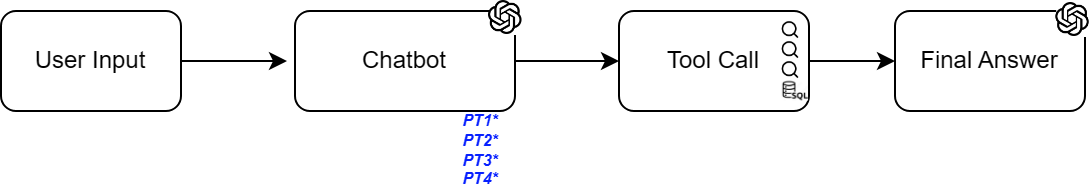
\includegraphics[width=0.8\textwidth]{images_exp2/diagrams/diagrama_linear_flow.png}
                    \caption{Linear-Flow architecture. PT1 indicates Prompt for Tool 1 and so on.}
                    \label{fig:diagrama_linear_flow}
                \end{figure}
           

            \subsubsection{Linear-Flow with Router}

                [VERSÃO 1]
                The Linear-Flow with Router architecture implements a sequential processing pipeline with routing, in order to divide and reduce tool instruction prompts. In this setup, questions first pass through a router that analyzes the query content and determines the most appropriate specialized node for the user query at hand. 
                
                [VERSÃO 2]
                The Linear-Flow with Router paradigm extends the basic linear flow by introducing a routing mechanism that enables the distribution of tool instruction prompts into specialized nodes with smaller prompts. User questions first pass through a router that determines the most appropriate specialized node. As illustrated in Figure~\ref{fig:diagrama_linear_w_router}, instead of a single node generating different types of retrieval queries, we have several nodes (or sub-queries), each with its own specialized tool. Each sub-query is then processed independently by separate tool invocations.
                    
                This approach offers several advantages:

                \begin{itemize}

                    \item \textbf{Increased Throughput:} By distributing sub-tasks across multiple tools, the system can handle more complex or multi-faceted user requests efficiently.
                    
                    \item \textbf{Specialization:} Each tool can be tailored to address a specific aspect of the user's query, allowing for more accurate and relevant results.
                    
                    \item \textbf{Scalability:} The architecture naturally supports scaling, as additional tools can be added to handle more sub-queries or specialized tasks.
                    
                \end{itemize}
                
                In practice, the router acts as an orchestrator, analyzing the user input and generating multiple targeted queries (PT1*, PT2*, PT3*, PT4* in the figure). These queries are dispatched to their respective tools, and the results are aggregated to form the final answer. This method is particularly effective for tasks that can be decomposed into independent components, such as multi-part questions or workflows requiring different types of expertise.
                
                Compared to the standard linear flow, the use of a router introduces additional complexity in query generation and result aggregation but enables a significant boost in system flexibility and performance.

                \begin{figure}[h]
                    \centering
                    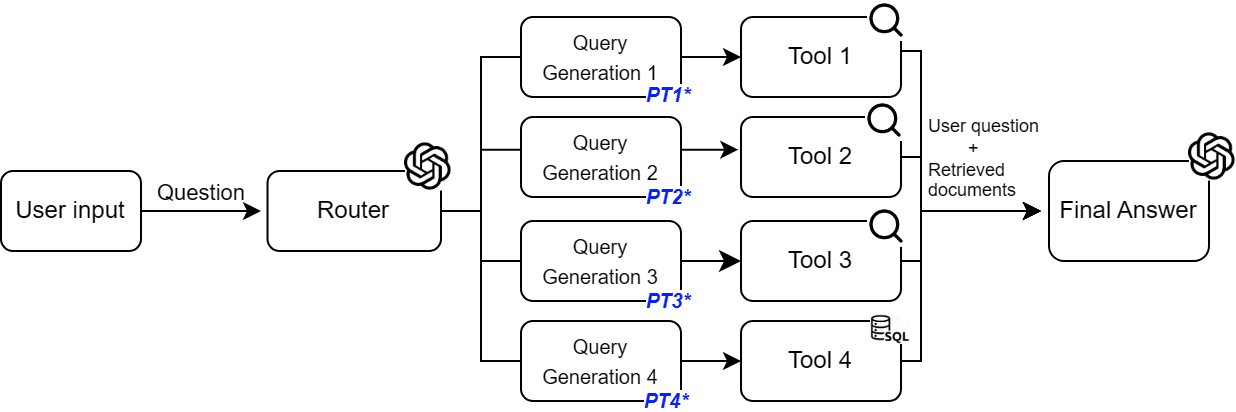
\includegraphics[width=0.8\textwidth]{images_exp2/diagrams/diagrama_linear_w_router.png}
                    \caption{Linear-Flow with Router architecture.}
                    \label{fig:diagrama_linear_w_router}
                \end{figure}
                
                

                
            \subsubsection{Single-Agent}

                The Single-Agent approach represents a centralized architecture where a single language model agent handles the entire question-answering process. This agent has access to the full suite of retrieval tools and knowledge sources, making independent decisions about which tools to invoke and how to synthesize information into coherent answers. The design emphasizes end-to-end reasoning within a unified context, allowing the model to maintain a consistent understanding throughout the process. This approach tests the capability of language models to manage complex workflows autonomously, balancing between exploration of different knowledge sources and focused answer generation without the overhead of inter-agent communication.
                
                \begin{figure}[h]
                    \centering
                    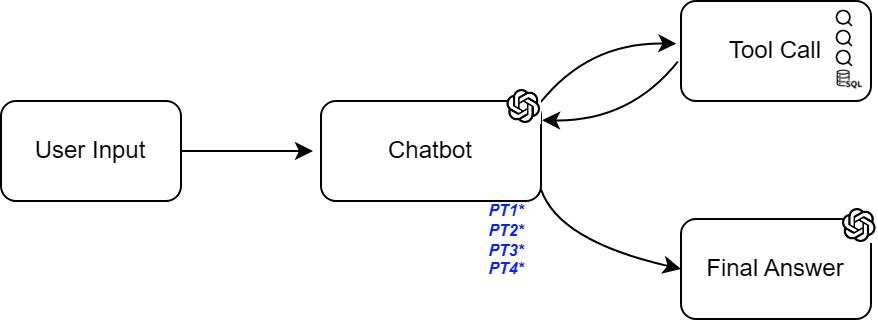
\includegraphics[width=0.5\textwidth]{images_exp2/diagrams/diagrama_single_agent.png}
                    \caption{Single-Agent architecture}
                    \label{fig:diagrama_single_agent}
                \end{figure}


            \subsubsection{Multi-Agent Supervisor}

                The Multi-Agent Supervisor setup implements a collaborative approach where multiple specialized agents work together under the coordination of a supervisor agent. Each specialized agent focuses on a specific domain of knowledge or reasoning skill, such as retrieval, analysis, or explanation generation. The supervisor agent orchestrates the collaboration, delegating subtasks to appropriate specialized agents, integrating their contributions, and ensuring coherence in the final answer. This architecture explores the potential benefits of distributed cognition, where complex reasoning is decomposed into manageable components handled by purpose-built agents. The framework includes mechanisms for resolving conflicts between agents and synthesizing potentially divergent perspectives into unified responses.

                \begin{figure}[h]
                    \centering
                    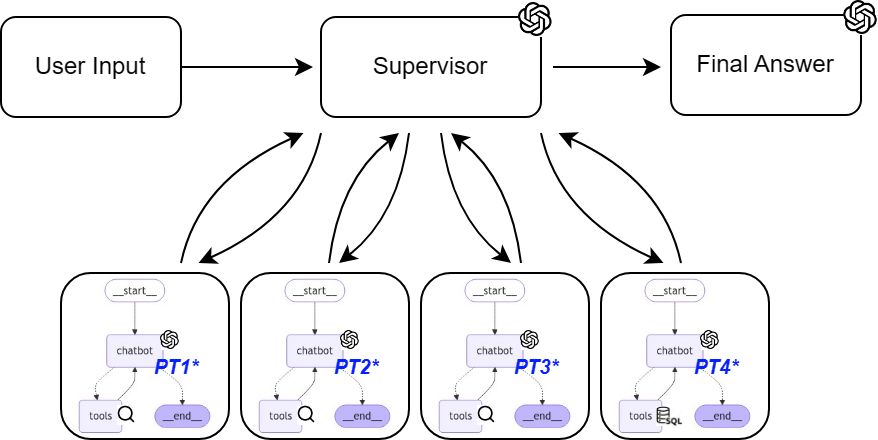
\includegraphics[width=0.6\textwidth]{images_exp2/diagrams/diagrama_multiagente_supervisor.png}
                    \caption{Multi-Agent setup with one supervisor and 4 specialist agents.}
                    \label{fig:diagrama_multiagente_supervisor}
                \end{figure}


                \textit{<insert table summarizing experimental setups and models here>}

        \subsection{Execution Details}

            The experiment was driven by a script without manual intervention during the evaluation process. A main execution loop systematically iterated through all combinations of questions, agent setups, and language models defined in the experimental design. 

            \subsubsection{Tool Integration and Knowledge Access}

            During execution, the agent systems accessed domain-specific knowledge through a standardized tool interface layer. This layer provided consistent access patterns across all experimental configurations, ensuring that differences in performance could be attributed to agent architecture rather than variations in knowledge availability. The tool integration framework supported a diverse range of knowledge access methods, including semantic search over unstructured text corpora, structured queries against relational databases, and specialized information extraction routines tailored to the oil well operations domain. Each tool invocation was executed within a controlled environment that captured performance metrics such as latency and resource utilization, providing additional dimensions for analysis beyond answer correctness. The standardization of tool interfaces across agent architectures was a critical design decision that enabled fair comparison while still allowing each architecture to implement its own strategy for tool selection and result interpretation.

            \subsubsection{Comprehensive Logging and Observability}

            A cornerstone of the experimental methodology was the implementation of comprehensive logging throughout the execution process. The system captured detailed records of each step in the question-answering workflow, from initial question parsing to final answer generation. These logs included intermediate reasoning steps, tool invocations with their inputs and outputs, and internal state transitions within the agent systems. All experimental artifacts were persisted in structured formats that facilitated both automated analysis and manual inspection. The logging system implemented a hierarchical organization that linked high-level metrics to the detailed execution traces that produced them, enabling root cause analysis of performance patterns. This observability infrastructure was essential for understanding not just what results were produced, but how and why different agent architectures arrived at their answers, providing insights into their reasoning processes and failure modes.

            \textit{<insert code snippet or pseudocode of main execution loop here>}

        \subsection{Evaluation Metrics}

            The evaluation of each experimental run is grounded in a comprehensive set of metrics designed to capture both the correctness and the quality of the system’s responses. Standard quantitative measures such as accuracy, precision, recall, and F1 score are calculated by comparing the answers generated by the agent systems to the established ground truth for each question. These metrics provide a multifaceted view of performance, indicating not only how often the system produces correct answers but also how well it balances false positives and false negatives.

            For questions that are open-ended or less amenable to binary correctness, the evaluation framework employs a confusion matrix approach. This allows for a more nuanced assessment, capturing partial correctness and the degree to which the system’s response overlaps with the expected content. Additionally, the methodology includes the calculation of the answer size ratio, which measures the verbosity of the generated answer relative to the ground truth. This metric helps to identify tendencies toward overly concise or excessively verbose responses, offering further insight into the models’ behavior and suitability for practical deployment.

        \subsection{Reproducibility}

            Ensuring reproducibility is a cornerstone of the experimental methodology. To this end, every aspect of the computational environment is meticulously documented. This includes recording the exact Python version used, as well as all package dependencies and their respective versions. Hardware specifications, such as processor type and available memory, are also logged to account for any potential influence on experimental outcomes.

            Beyond the environment, the system systematically records all configuration parameters relevant to each experimental run. This encompasses model names, hyperparameters, and dataset paths, as well as any other settings that might affect the results. By maintaining this comprehensive record, the methodology enables other researchers to replicate the experiments precisely or to build upon them with confidence that baseline conditions are well understood and controlled.

        \subsection{Limitations}

            While the experimental methodology strives for rigor and comprehensiveness, several limitations must be acknowledged. One key limitation concerns the coverage of the dataset: although the question set is carefully curated to represent a broad range of operational scenarios, it may not capture the full diversity of real-world challenges encountered in oil well operations. Similarly, the models and agent architectures evaluated are constrained by the available computational resources and the current state of language modeling technology, which may limit their ability to generalize beyond the scenarios tested.

            Another limitation arises from the reliance on ground truth answers, which, despite expert validation, may still reflect subjective judgments or incomplete information in certain cases. Furthermore, the evaluation metrics, while robust, may not fully capture qualitative aspects of answer usefulness or clarity, especially in highly technical or ambiguous situations. Recognizing these limitations is essential for interpreting the results and for guiding future research aimed at addressing these gaps.

        \subsection{Summary}

            This methodology provides a systematic framework for comparing different agent architectures and large language models in the context of complex question answering for oil well operations. By integrating rigorous evaluation metrics, robust reproducibility practices, and a clear acknowledgment of limitations, the approach enables meaningful insights into the strengths and weaknesses of various system designs. The findings derived from this methodology can inform both the deployment of language model agents in operational settings and the ongoing development of more capable and reliable AI systems for specialized industrial domains.


    \section{Resultados e Discussão}

        
        \subsection{Performance}

        
            [GERAR TEXTO AQUI]

            ... \cite{Antoniak2016}

            ...
            
            \begin{figure}[h]
                \centering              
                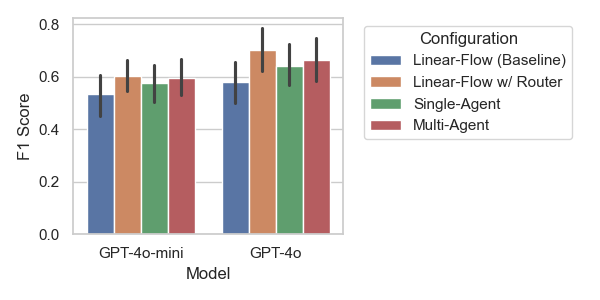
\includegraphics[width=0.50\textwidth]{images_exp2/bar_best_f1_by_model_and_configuration.png}
                \caption{Best F1 score by model and configuration.}
                \label{fig:best_f1_by_model_and_configuration}
            \end{figure}


            ...

            
            \begin{figure}[h!]
                \centering              
                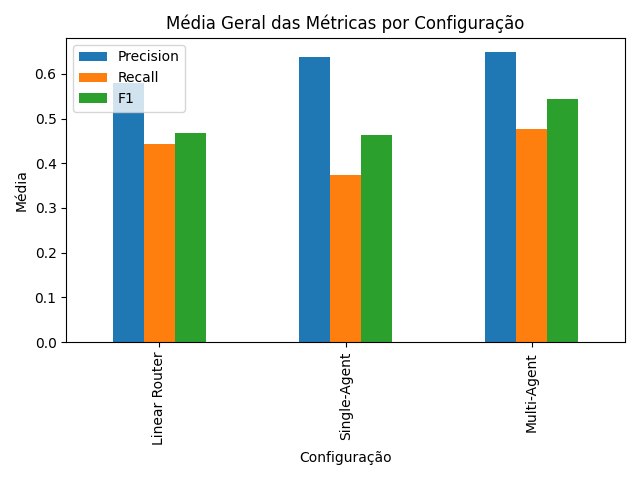
\includegraphics[width=0.75\textwidth]{images_part_2/media_geral_por_configuracao.png}
                \caption{Precisão, recall e f1 por configuração.             [GERAR GRÁFICO NOVO AQUI]}
                \label{fig:media_geral_por_configuracao}
            \end{figure}


            ...
            
            ...

            ...
        
            \subsubsection{F1 Score}
            
                
                [GERAR TEXTO AQUI]

                ...

                ...

                ...
                
                % \begin{figure}
                %     \centering
                %     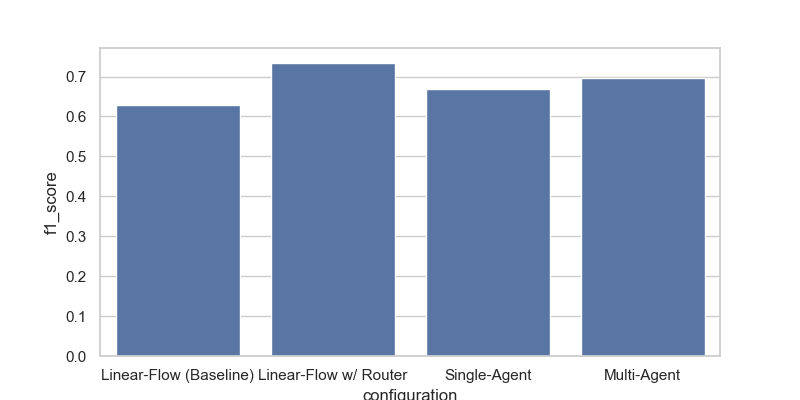
\includegraphics[width=0.5\linewidth]{images_exp2/bar_avg_f1_by_configuration.png}
                %     \caption{Average F1 by RAG architecture.}
                %     \label{fig:enter-label}
                % \end{figure}

                % \begin{figure}
                %     \centering
                %     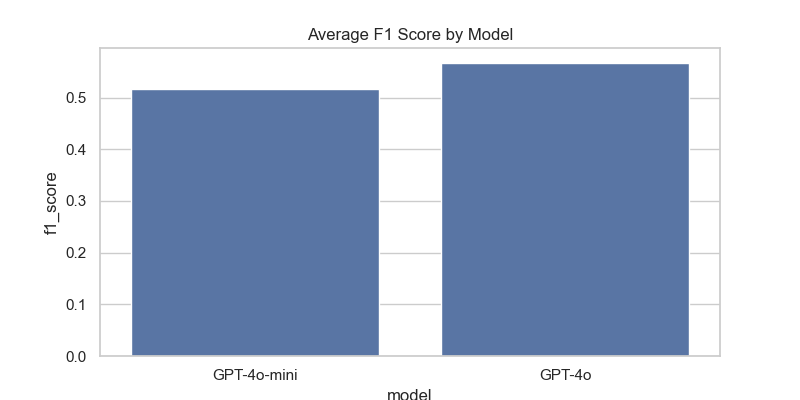
\includegraphics[width=0.5\linewidth]{images_exp2/bar_avg_f1_by_model.png}
                %     \caption{Average F1 Score by language model.}
                %     \label{fig:enter-label}
                % \end{figure}            
                \begin{figure}[h]
                \centering
                \begin{minipage}{0.45\textwidth}
                    \centering
                    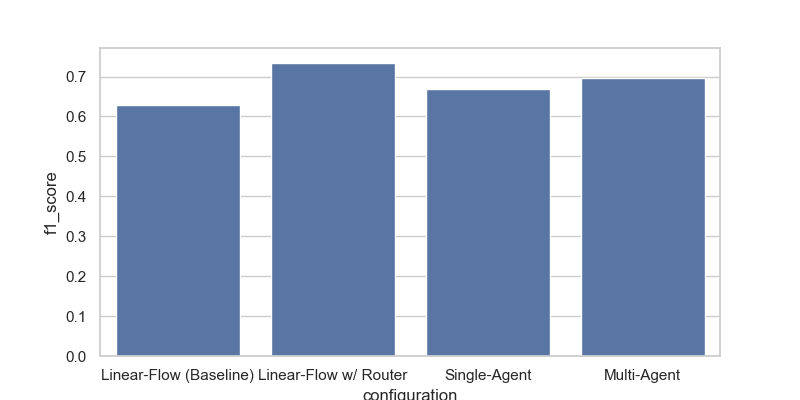
\includegraphics[width=\textwidth]{images_exp2/bar_avg_f1_by_configuration.png}
                    \caption{Image 1 caption}
                    \label{fig:image1}
                \end{minipage}
                \hfill
                \begin{minipage}{0.45\textwidth}
                    \centering
                    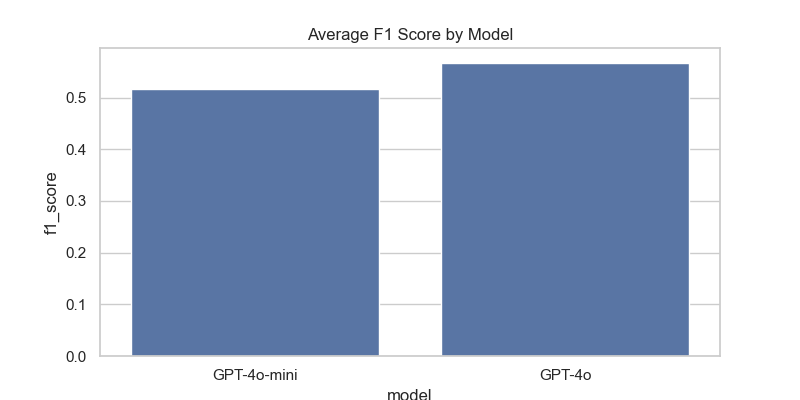
\includegraphics[width=\textwidth]{images_exp2/bar_avg_f1_by_model.png}
                    \caption{Image 2 caption}
                    \label{fig:image2}
                \end{minipage}
                \end{figure}
                
                
                [GERAR TEXTO AQUI]

                ...

                ...

                ...
                % \begin{figure}[h!]
                %     \centering              
                %     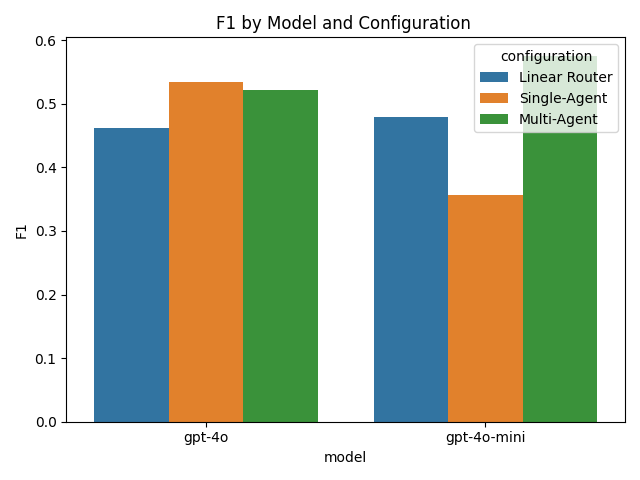
\includegraphics[width=0.75\textwidth]{images_part_2/model_f1_model_configuration.png}
                %     \caption{F1 Score por modelo e configuração.}
                %     \label{fig:aaaa}
                % \end{figure}
                \begin{figure}
                    % \centering
                    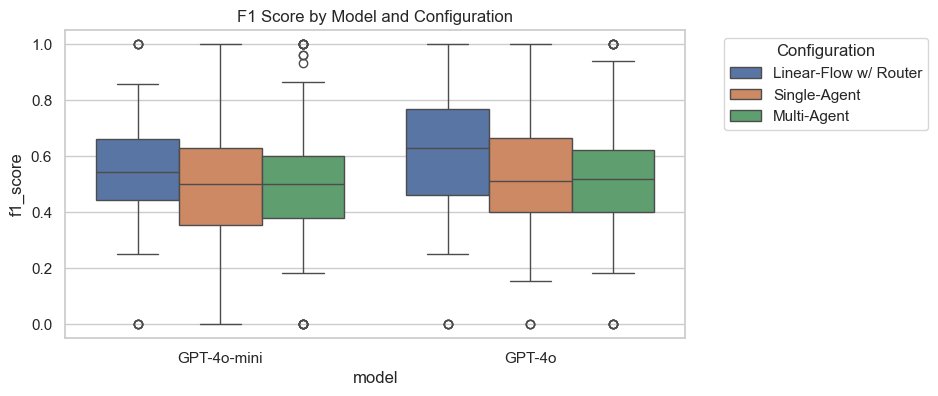
\includegraphics[width=1.1\linewidth]{images_exp2/f1_score_by_model_and_configuration.png}
                    \caption{F1 Score distribution by model and configuration of agents}
                    \label{fig:f1_score_by_model_and_configuration}
                \end{figure}
                    
                [GERAR TEXTO AQUI]

                ...

                ...

                ...
                
                
                \begin{figure}
                    \centering
                    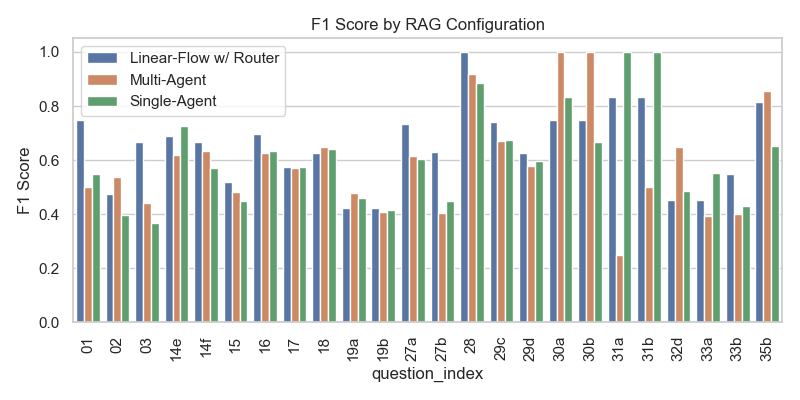
\includegraphics[width=1\linewidth]{images_exp2/best_f1_by_question_index_and_configuration.png}
                    \caption{Enter Caption}
                    \label{fig:best_f1_by_question_index_and_configuration}
                \end{figure}
                
                [GERAR TEXTO AQUI]

                ...

                ...

                ...
                
                % \begin{figure}[h!]
                %     \centering              
                %     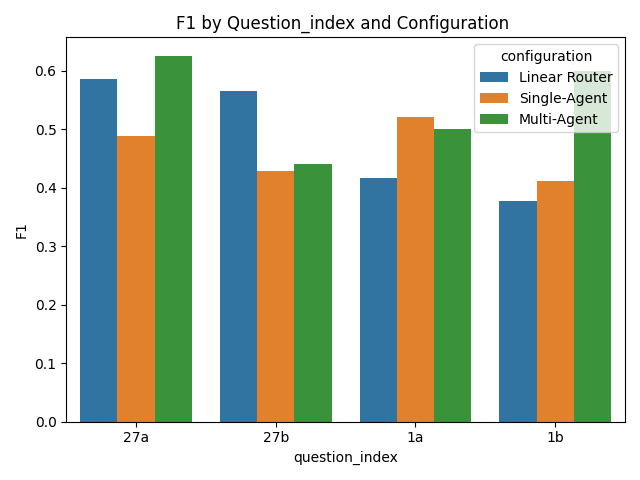
\includegraphics[width=0.75\textwidth]{images_part_2/question_f1_question_index_configuration.png}
                %     \caption{F1 Score por pergunta e configuração.}
                %     \label{fig:aaaa}
                % \end{figure}


                [GERAR TEXTO AQUI]

                ...

                ...
                
                ...

                
                \begin{figure}
                    \centering
                    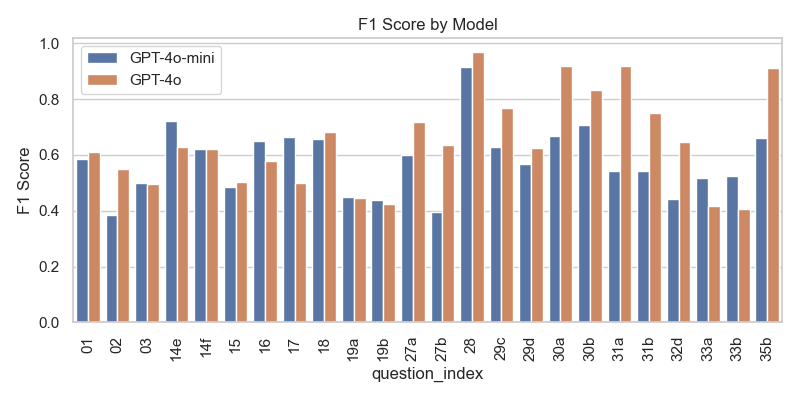
\includegraphics[width=1\linewidth]{images_exp2/best_f1_by_question_index_and_model.png}
                    \caption{Enter Caption}
                    \label{fig:best_f1_by_question_index_and_model}
                \end{figure}


            \subsubsection{Precisão}

                [GERAR TEXTO AQUI]

                ...

                ...

                ...

                \begin{figure}[h!]
                    \centering              
                    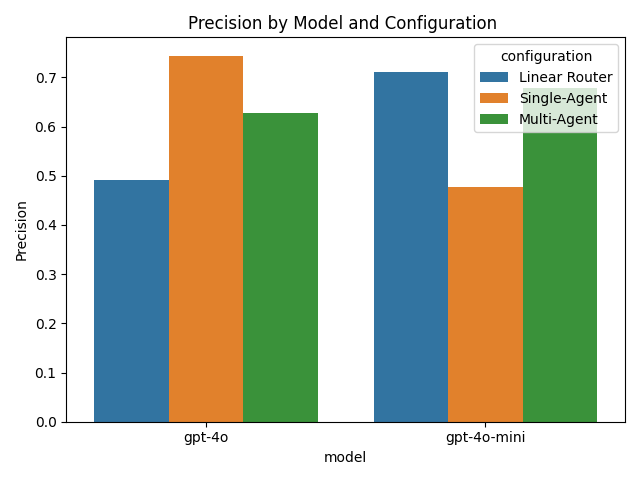
\includegraphics[width=0.75\textwidth]{images_part_2/model_precision_model_configuration.png}
                    \caption{Precisão por modelo e configuração.}
                    \label{fig:model_precision_model_configuration}
                \end{figure}
                
                [GERAR TEXTO AQUI]

                ...

                ...

                ...

                \begin{figure}[h!]
                    \centering              
                    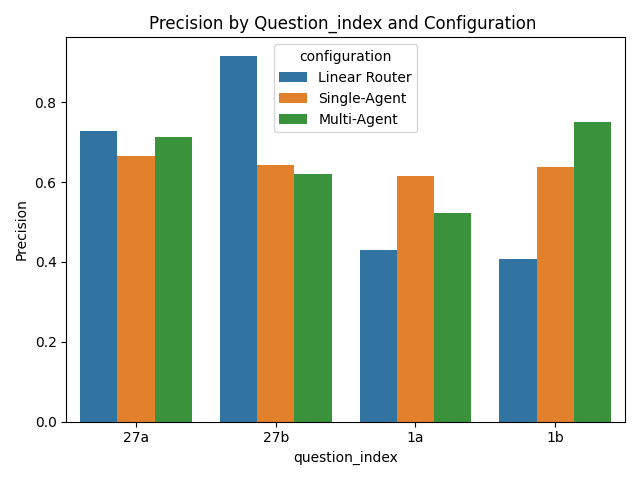
\includegraphics[width=0.75\textwidth]{images_part_2/question_precision_question_index_configuration.png}
                    \caption{Precisão por pergunta e configuração.}
                    \label{fig:question_precision_question_index_configuration}
                \end{figure}    

                [GERAR TEXTO AQUI]

                ...

                ...

            
            \subsubsection{Recall}
            
                [GERAR TEXTO AQUI]

                ...

                ...
                
                \begin{figure}[h!]
                    \centering              
                    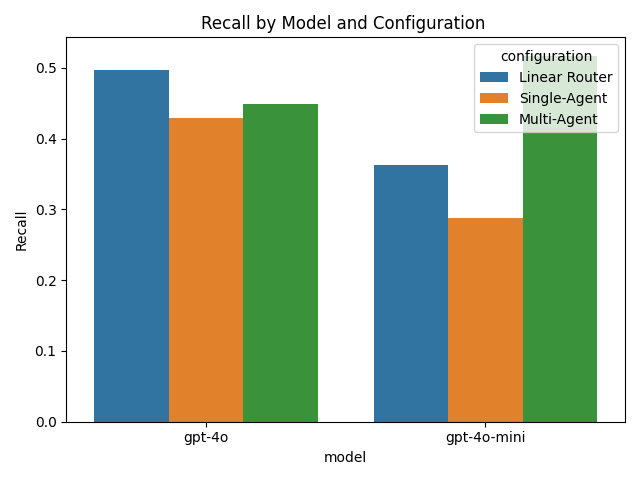
\includegraphics[width=0.75\textwidth]{images_part_2/model_recall_model_configuration.png}
                    \caption{Recall por modelo e configuração.}
                    \label{fig:aaaa}
                \end{figure}

                [GERAR TEXTO AQUI]

                ...

                ...

                ...
                
                \begin{figure}[h!]
                    \centering              
                    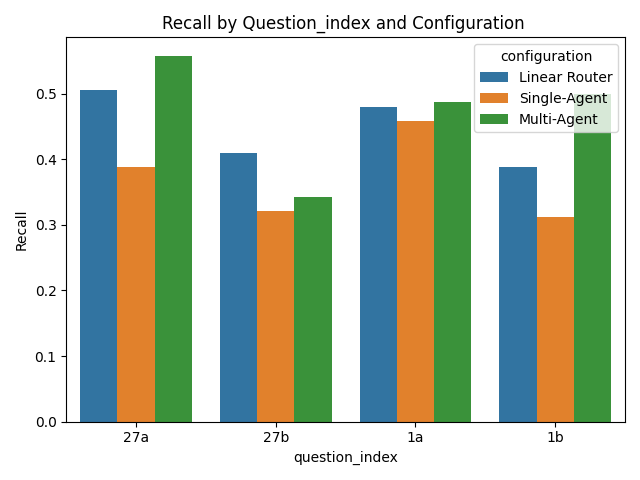
\includegraphics[width=0.75\textwidth]{images_part_2/question_recall_question_index_configuration.png}
                    \caption{Recall por pergunta e configuração.}
                    \label{fig:question_recall_question_index_configuration}
                \end{figure}

                [GERAR TEXTO AQUI]

                ...

                ...
            

        \subsection{Linear-Flow}


            In this setup, the user’s query is handled by a single LLM step, which carries all the instructions (PT1, PT2, PT3 and PT4, as depicted in \ref{fig:diagrama_linear_flow}) required for the generation of various types of search queries. These instruction prompts are often quite long, as they are carefully crafted to produce high-quality queries for the vector store. Due to the aggregation of all instruction prompts within a single LLM invocation, the resulting context becomes notably extensive. This can lead to performance degradation as the context length increases [O QUE PODE SER VISTO NO GRAFICO TAL EM CONTRASTE COM O SETUP TAL QUE DIVIDE OS PROMPTS EM PARTES]. 
            
            ...

            ...
            
            ...

        \subsection{Linear-Flow with Router}

            [GERAR TEXTO AQUI]

            ...

            ...
            
            ...

        \subsection{Single-Agent}

            [GERAR TEXTO AQUI]

            ...

            ...
            
            ...
        
        \subsection{Multi-Agent}

            [GERAR TEXTO AQUI]

            ...
            
            ...
            
            ...
